\documentclass[aspectratio=169]{beamer}
\usetheme{default}
\usecolortheme{default}
\usepackage{graphicx}
\usepackage{subcaption}

% Title information
\title[Neural Population Geometry]{Neural Population Geometry}
\subtitle{ME 225NN, Winter 2025}
\author[Acosta \& Skaza]{Santiago Acosta \& Jonathan Skaza}
\institute[UCSB]{Dynamical Neuroscience Graduate Program\\University of California, Santa Barbara}
\date{}

\begin{document}

% Title slide
\begin{frame}
    \titlepage
\end{frame}

% Outline slide
\begin{frame}{Outline}
    \tableofcontents
\end{frame}

% Introduction section
\section{Introduction}

\begin{frame}{Problem Description \& Motivation}
    \begin{itemize}
        \item Advances in recording techniques: thousands to millions of neurons simultaneously
        \item Challenges in studying large neural populations:
        \begin{itemize}
            \item Neurons respond to multiple variables
            \item Traditional tuning-based analyses have limitations
        \end{itemize}
        \item Shift from single-neuron tuning to geometric approaches
        \item Neural computations arise from structured, high-dimensional activity patterns
    \end{itemize}
\end{frame}

\begin{frame}{Neural Manifolds}
    \begin{itemize}
        \item Neural manifolds: low-dimensional geometric structures embedded in high-dimensional neural state space
        \item Key properties: dimensionality, curvature, and separability
        \item Provide insights into computational principles governing neural networks
        \item Framework has provided mechanistic insights into:
        \begin{itemize}
            \item Perception
            \item Decision-making
            \item Motor control
            \item Cognition
        \end{itemize}
    \end{itemize}
\end{frame}

\begin{frame}{Bridging Biological and Artificial Neural Networks}
    \begin{itemize}
        \item Neural population geometry bridges biological and artificial neural networks
        \item Shared representational structures support efficient computation
        \item Geometric properties shape information encoding and processing
        \item Geometric perspective reveals how neural populations achieve:
        \begin{itemize}
            \item Robustness
            \item Efficiency
            \item Scalability
        \end{itemize}
    \end{itemize}
\end{frame}

% Preliminaries section
\section{Preliminaries}

\begin{frame}{Neural State Space \& Population Activity}
    \begin{columns}
        \column{0.5\textwidth}
        \begin{itemize}
            \item Neural state space: each axis represents a single neuron
            \item Repeated stimulus presentations create point clouds
            \item Neuronal variability induces fluctuations
            \item Manifolds emerge from stimulus responses
        \end{itemize}
        
        \column{0.5\textwidth}
        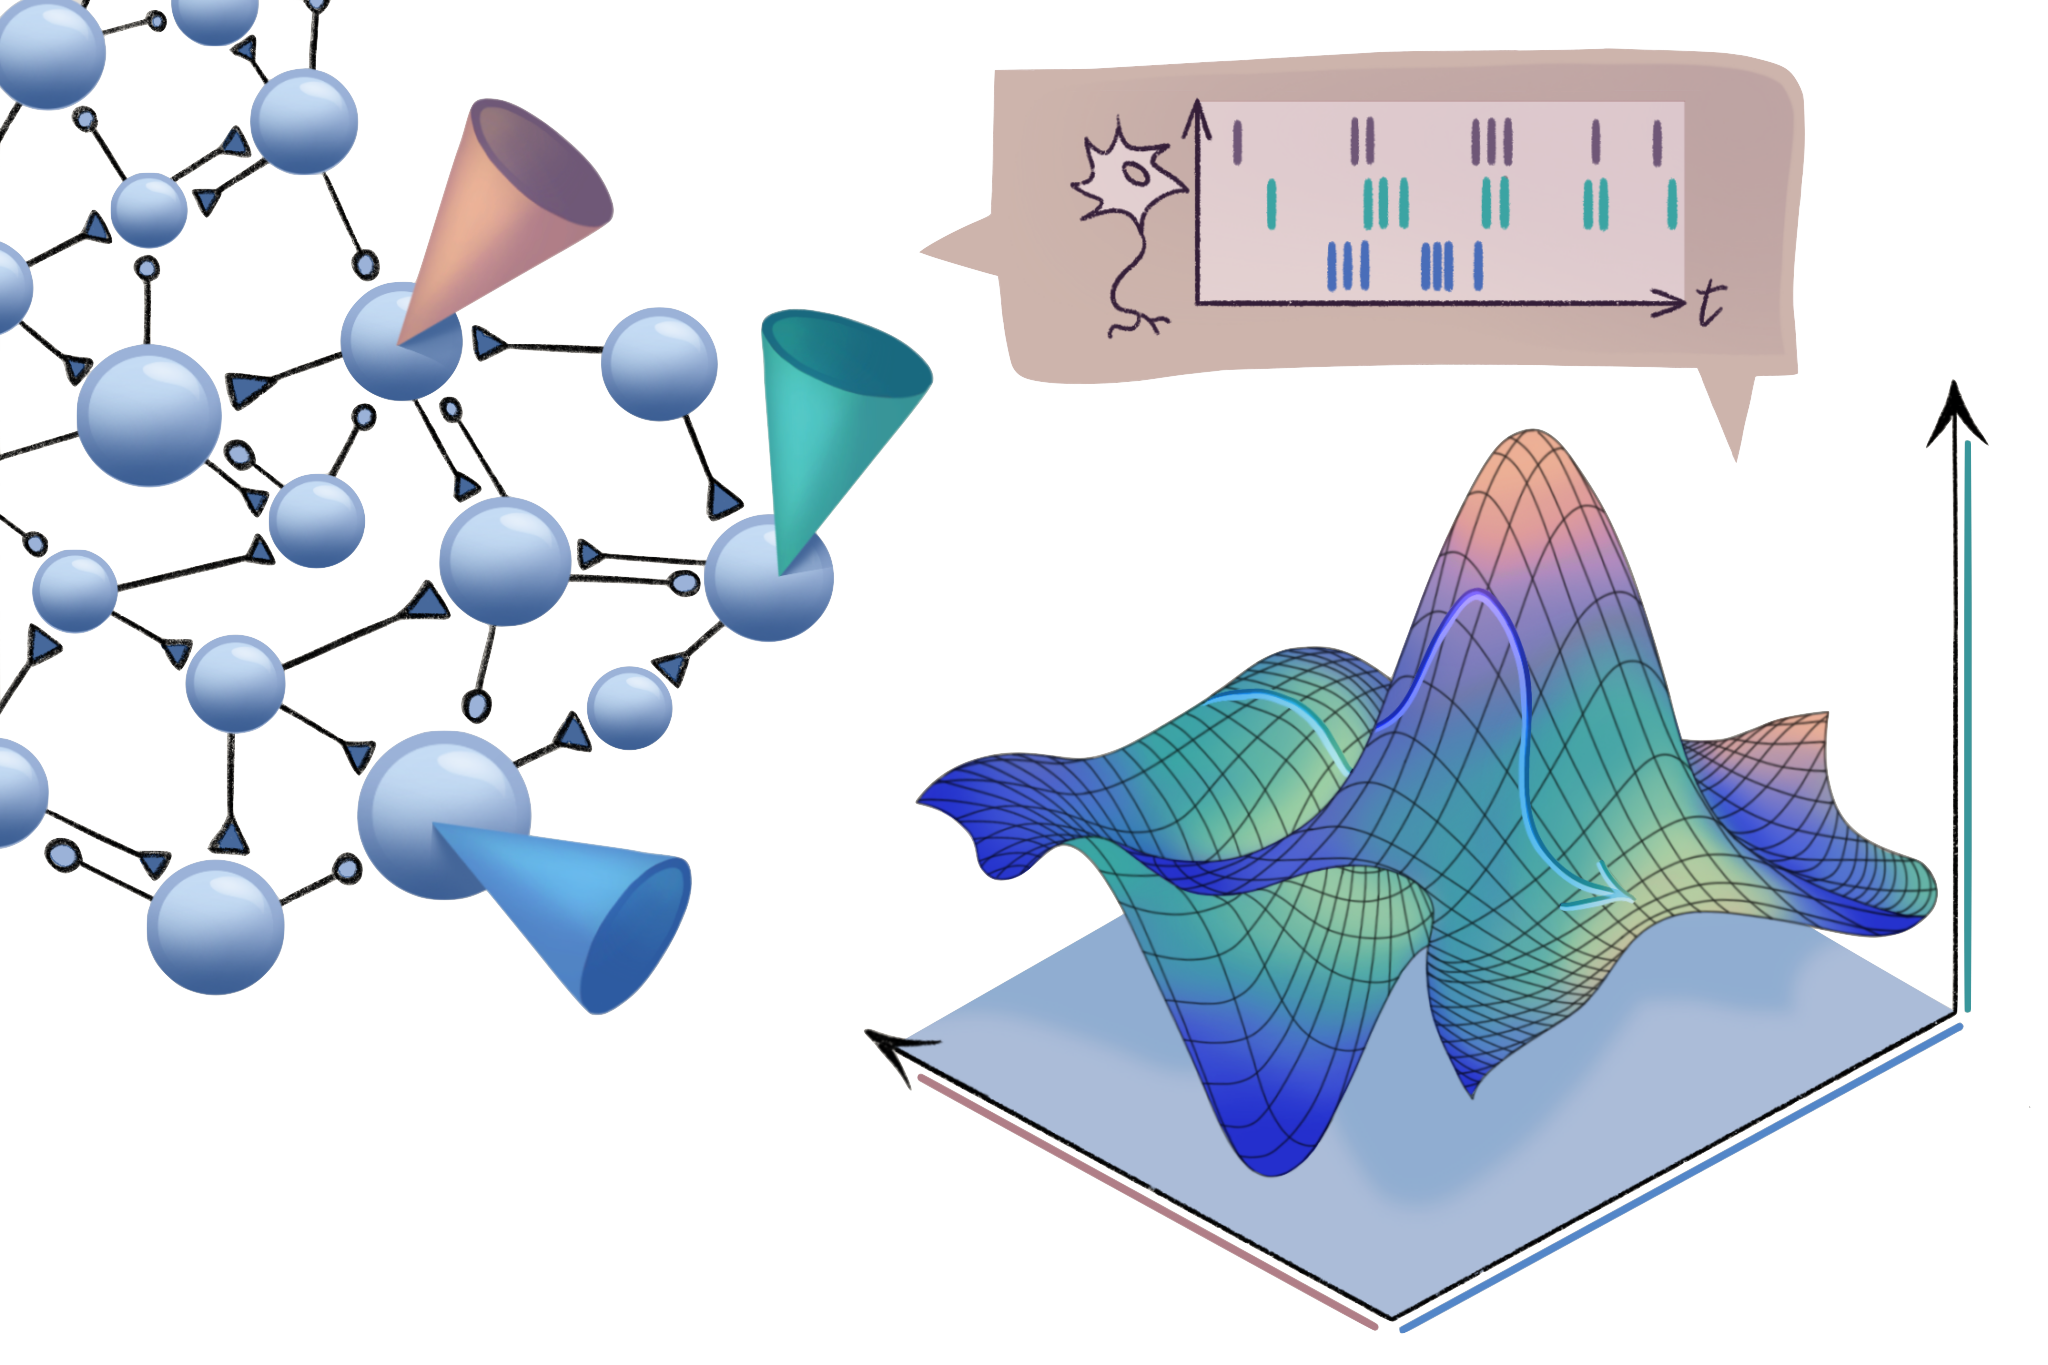
\includegraphics[width=\textwidth]{manifold_schematic.png}
    \end{columns}
\end{frame}

% Neural Population Geometry section
\section{Neural Population Geometry}

\begin{frame}{Key Concepts in Neural Population Geometry}
    \begin{itemize}
        \item Population-level representations vs. single-neuron tuning
        \item Geometric transformations of neural manifolds
        \item Dimensionality and information encoding
        \item Manifold separability and computational capabilities
        \item Curvature and computational constraints
    \end{itemize}
\end{frame}

% Simulation section
\section{Simulation}

\begin{frame}{Artificial Neural Networks}
    \begin{itemize}
        \item Demonstration of geometric structures in neural representations
        \item Simulation experiment: encoding circular variables
        \item Illustrates how topological structures naturally emerge
    \end{itemize}
    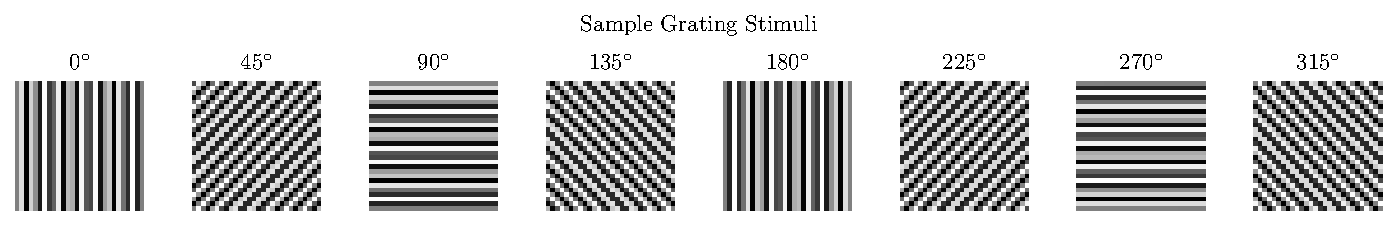
\includegraphics[width=0.7\textwidth]{results/grating_samples.pdf}
    \captionof{figure}{Sample grating stimuli at different orientations}
\end{frame}

\begin{frame}{Circular Manifold Experiment}
    \begin{itemize}
        \item CNN trained to predict orientation of visual grating stimuli
        \item Analogous to orientation selectivity in visual cortex
        \item Sinusoidal gratings at orientations from 0° to 360°
        \item Architecture: convolutional layers + fully connected layers
        \item 32-dimensional latent space analyzed for geometric properties
        \item Trained to predict sine and cosine components (handles circular topology)
    \end{itemize}
\end{frame}

\begin{frame}{Results: Circular Manifold}
    \begin{columns}
        \column{0.5\textwidth}
        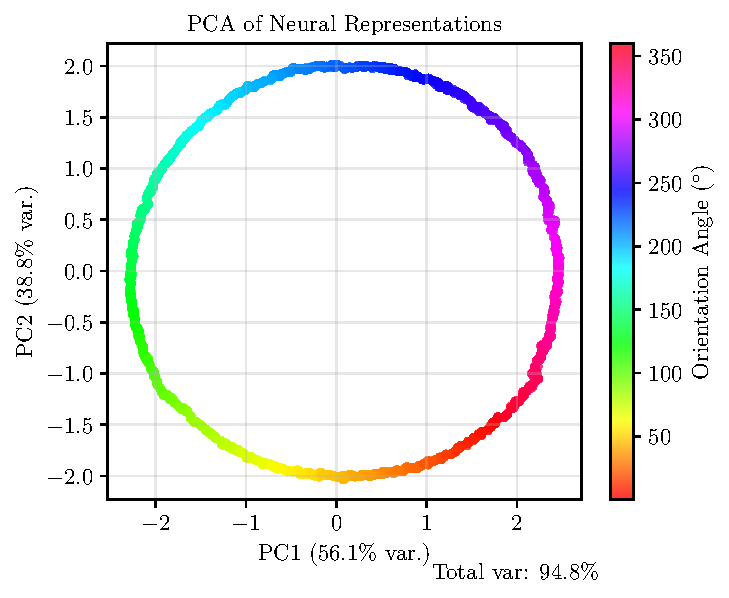
\includegraphics[width=\textwidth]{results/pca_latent_space.pdf}
        \captionof{figure}{PCA of the latent space}
        
        \column{0.5\textwidth}
        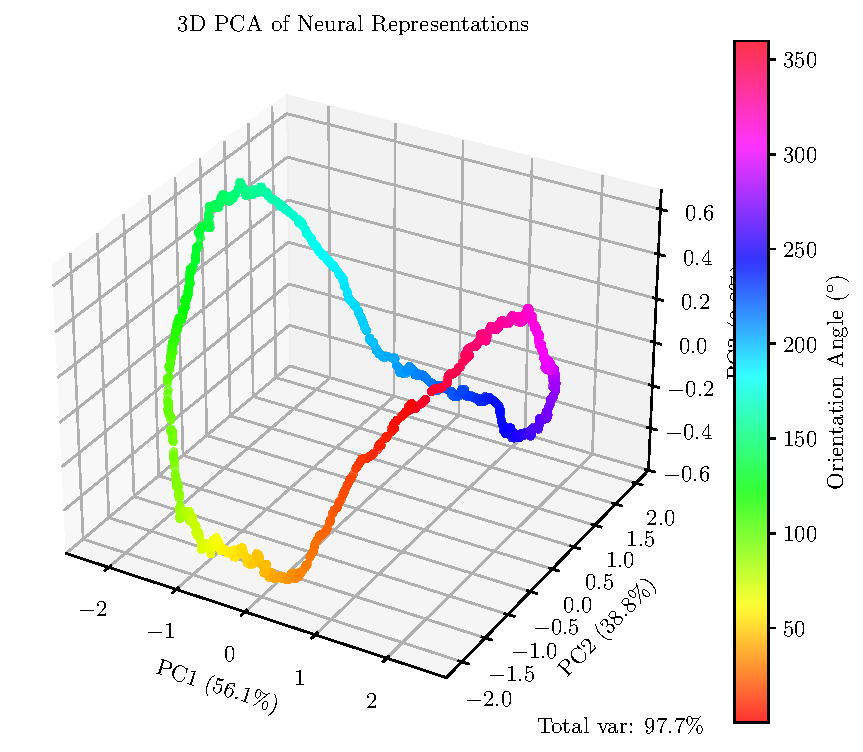
\includegraphics[width=\textwidth]{results/3d_manifold.pdf}
        \captionof{figure}{3D visualization of the manifold}
    \end{columns}
    \vspace{0.5cm}
    \begin{itemize}
        \item Circular manifold emerged in latent space
        \item Similar orientations positioned close together
        \item Orientation space represented as continuous ring
    \end{itemize}
\end{frame}

\begin{frame}{Key Principles Demonstrated}
    \begin{itemize}
        \item \textbf{Manifold structure}: Low-dimensional manifold (circle) embedded in high-dimensional space
        \item \textbf{Topological correspondence}: Manifold topology matches task space topology
        \item \textbf{Continuous representation}: Similar stimuli mapped to nearby points
        \item \textbf{Dimensionality reduction}: High-dimensional input compressed to essential variables
    \end{itemize}
    \vspace{0.5cm}
    \begin{block}{Insight}
        Circular topology emerged naturally without explicit constraints—the network discovered this efficient representation on its own
    \end{block}
\end{frame}

\begin{frame}{Biological Neural Networks}
    % Placeholder for biological neural networks content
    \begin{itemize}
        \item Application of geometric principles to biological neural data
        \item Comparison with artificial neural network findings
        \item Insights into biological neural computation
    \end{itemize}
\end{frame}

% Conclusion section
\section{Conclusion}

\begin{frame}{Conclusion}
    \begin{itemize}
        \item Neural population geometry provides powerful framework for analyzing neural activity
        \item Geometric principles describe population-level representations
        \item Approach yields mechanistic insights across multiple domains
        \item Bridges biological and artificial neural networks
        \item Geometric perspective deepens understanding of neural computation
    \end{itemize}
\end{frame}

\begin{frame}{References}
    \begin{thebibliography}{10}
        \bibitem{demas2021high} Demas, J. et al. (2021). High-speed, cortex-wide volumetric recording of neuroactivity.
        \bibitem{yuste2015neuron} Yuste, R. (2015). From the neuron doctrine to neural networks.
        \bibitem{saxena2019towards} Saxena, S. \& Cunningham, J. P. (2019). Towards the neural population doctrine.
        \bibitem{chung2021neural} Chung, S. \& Abbott, L. F. (2021). Neural population geometry: An approach for understanding biological and artificial neural networks.
        \bibitem{Perich2024} Perich, M. G. et al. (2024). Neural manifolds and population dynamics.
    \end{thebibliography}
\end{frame}

\end{document} 